% ===========================================================================
% main_raccefyn.tex
% Revista de la Academia Colombiana de Ciencias Exactas, Físicas y Naturales
% Sección: Ciencias Físicas (Electromagnetismo, Problemas Inversos y Biofísica)
% Formato oficial: Styles_ACCEFN.sty (biblatex + biber, estilo APA 7)
% ===========================================================================
\documentclass[9pt]{article}

% ── Idioma y codificación ─────────────────────────────────────────────────
\usepackage[spanish,es-tabla,es-nodecimaldot]{babel}
\usepackage[T1]{fontenc}
\usepackage{csquotes}

% ── Matemáticas (cargado antes de Styles_ACCEFN para evitar colisión \iint) ─
\usepackage{amsmath}
\usepackage{bm}

% ── Márgenes oficiales RACCEFYN ───────────────────────────────────────────
\usepackage[left=6.9cm, right=1.9cm, top=3.1cm, bottom=2.3cm]{geometry}

% ── Hoja de estilos oficial RACCEFYN ──────────────────────────────────────
\usepackage{Styles_ACCEFN}

% ── Delimitadores de autor en bibliografía sin 'and' ──────────────────────
\DeclareDelimFormat[bib]{finalnamedelim}{%
  \ifthenelse{\value{listcount}>\maxprtauth}
    {}
    {\ifthenelse{\value{liststop}>2}
       {\finalandcomma\addspace}
       {\addspace}}}
\DeclareDelimFormat[bib]{finalnamedelim:apa:family-given}{%
  \ifthenelse{\value{listcount}>\maxprtauth}
    {}
    {\ifthenelse{\ifcurrentname{groupauthor}\AND\value{liststop}=2}
     {\addspace}
     {\finalandcomma\addspace}}}

% ── Apellidos en negrita en citas y bibliografía (norma RACCEFYN) ─────────
\renewcommand*{\mkbibnamefamily}[1]{\textbf{#1}}
\renewcommand*{\mkbibnamegiven}[1]{#1}
\renewcommand*{\mkbibnameprefix}[1]{#1}
\renewcommand*{\mkbibnamesuffix}[1]{#1}

% ── Paquetes adicionales de soporte ───────────────────────────────────────
\usepackage{multirow}
\usepackage{array}
\usepackage{xcolor}
\usepackage{url}

% ── Ruta de figuras ───────────────────────────────────────────────────────
\graphicspath{{./figures/}{../results/paper2_artifacts/}{./}}

% ── Archivo de bibliografía ───────────────────────────────────────────────
\addbibresource{references_raccefyn.bib}

% ── Encabezado con título corto (Running title <= 10 palabras, <= 50 caract.: 7 palabras, 47 caract.)
\fancyhead[L]{\fontsize{8}{10}\selectfont\textit{Tomografía electro-térmica por PINN y biocalor}}

% ── Metadatos del documento PDF ───────────────────────────────────────────
\hypersetup{
    pdftitle={Tomografía de propiedades eléctricas por convección-reacción diferenciable y modelado de biocalor de Pennes mediante redes informadas por la física},
    pdfauthor={Yerson Hernando León-Montañez},
    pdfkeywords={ecuación de convección-reacción; ecuación de biocalor de Pennes; tomografía de propiedades eléctricas; redes PINN; dosis térmica CEM43; hipoperfusión tumoral}
}

\definecolor{raccefyngray}{RGB}{110,110,110}
\emergencystretch=2em

% ===========================================================================
\begin{document}

% ── Área de conocimiento y Título corto (metadatos editoriales RACCEFYN) ──
\noindent{\fontsize{8.5}{10}\selectfont\textbf{Sección:} Ciencias Físicas \quad|\quad \textbf{Título corto:} Tomografía electro-térmica por PINN y biocalor}\\[0.25cm]

% ── Título en español (<= 30 palabras, <= 165 caracteres: 20 palabras, 163 caracteres)
% ── e inglés debajo en gris según plantilla oficial RACCEFYN (13 palabras, 126 caracteres) ──
\title{{\fontsize{13.0}{15.0}\selectfont Tomografía de propiedades eléctricas por convección-reacción diferenciable y modelado de biocalor de Pennes mediante redes informadas por la física}\\[0.25cm]
{\fontsize{11.0}{13.0}\selectfont\color{raccefyngray} Differentiable convection-reaction electrical properties tomography and Pennes bioheat modeling via physics-informed networks}\\[0.55cm]}

% ── Autoría con apellidos unidos por guion, afiliación y ORCID ────────────
\author[1,*]{Yerson Hernando León-Montañez \orcidlink{0009-0000-4439-8661}}
\affil[1]{\fontsize{8}{9}\selectfont Facultad de Ingeniería, Maestría en Inteligencia Artificial, Universidad de La Salle, Bogotá, Colombia}
\affil[*]{\fontsize{8}{9}\selectfont Correspondencia: yeleon36@unisalle.edu.co; yelemo777@gmail.com; Tel: +57 3057278736}

\date{}
\maketitle

% ===========================================================================
% RESUMEN (<= 250 palabras, un solo párrafo estructurado)
% ===========================================================================
\begin{abstract}
\noindent La Tomografía de Propiedades Eléctricas por Resonancia Magnética (MR-EPT) basada en la ecuación de Helmholtz trunca los gradientes espaciales de conductividad ($\nabla\sigma \approx \mathbf{0}$), provocando una subestimación del $-18\%$ al $-23\%$ en tumores gliales y colapsando el valor dieléctrico del líquido cefalorraquídeo ventricular en un $-46\%$. Asimismo, calcular únicamente la tasa de absorción específica ($\text{SAR}$) omite la termorregulación vascular. En este trabajo formulamos \textbf{ElectroThermalMRIPINN}, un marco acoplado multi-física que supera estas limitaciones mediante tres contribuciones: (1) resolución diferenciable exacta de la ecuación de Convección-Reacción sobre representaciones implícitas periódicas (SIREN) evaluando analíticamente $\nabla_m\sigma\cdot\nabla_m\phi^+$ vía \texttt{autograd} sin difusión artificial; (2) acoplamiento transitorio con la ecuación diferencial parabólica de Biocalor de Pennes ($0\text{--}30\text{ min}$) para predecir temperatura absoluta en $^\circ\text{C}$ y dosis térmica $\text{CEM}_{43}$ bajo hipoperfusión tumoral ($\omega_{b,\text{tumor}} = 0.25\,\omega_{b,\text{sano}}$); y (3) balanceo auto-adaptativo por norma de gradientes (GradNorm). En evaluaciones numéricas multi-campo ($1.5\text{ T}$, $3.0\text{ T}$, $7.0\text{ T}$, $N=5$) y validaciones en la estación PACS Electro-Térmica 2.0 ($R=4\times, 8\times$), el método reduce el error $\text{NRMSE}(\sigma)$ de $35.2\%$ a $19.7\%\text{--}20.57\%$, recupera fielmente la conductividad del glioma ($1.172\text{--}1.21\text{ S/m}$) y de los ventrículos ($1.595\text{--}1.62\text{ S/m}$ frente a $0.86\text{ S/m}$ en Helmholtz), y demuestra cómo la absorción electromagnética genera trampas térmicas intratumorales de $39.47\text{--}39.59^\circ\text{C}$ ($\text{CEM}_{43} = 0.144\text{--}0.167\text{ min}$, alerta IEC de nivel controlado), contrastando con controles basales seguros en adquisiciones humanas reales de cerebro, rodilla, tórax y abdomen.
\end{abstract}

\noindent\textbf{Palabras clave:} ecuación de convección-reacción; ecuación de biocalor de Pennes; tomografía de propiedades eléctricas; redes PINN; dosis térmica CEM43; hipoperfusión tumoral.

\vspace{0.35cm}

% ===========================================================================
% ABSTRACT (<= 250 words, single structured paragraph)
% ===========================================================================
\renewcommand{\abstractname}{Abstract}
\begin{abstract}
\noindent Helmholtz-based Magnetic Resonance Electrical Properties Tomography (MR-EPT) assumes locally homogeneous tissues ($\nabla\sigma \approx \mathbf{0}$), systematically underestimating glioma conductivity by $-18\%$ to $-23\%$ and truncating ventricular cerebrospinal fluid conductivity by $-46\%$. Moreover, relying strictly on specific absorption rate ($\text{SAR}$) ignores microvascular thermoregulation. In this study, we propose \textbf{ElectroThermalMRIPINN}, a coupled multi-physics framework addressing these limitations via three contributions: (1) exact differentiable solution of the Convection-Reaction partial differential equation on periodic implicit neural representations (SIREN), analytically evaluating $\nabla_m\sigma\cdot\nabla_m\phi^+$ via automatic differentiation without artificial viscosity; (2) transient coupling with Pennes' parabolic bioheat transfer equation ($0\text{--}30\text{ min}$) to predict absolute temperature maps in $^\circ\text{C}$ and cumulative thermal dose ($\text{CEM}_{43}$) under necrotic tumor hypoperfusion ($\omega_{b,\text{tumor}} = 0.25\,\omega_{b,\text{healthy}}$); and (3) gradient-norm dynamic balancing (GradNorm). Multi-field numerical evaluations ($1.5\text{ T}$, $3.0\text{ T}$, $7.0\text{ T}$, $N=5$) and clinical PACS 2.0 validations under $R=4\times$ and $8\times$ acceleration demonstrate that the proposed method lowers global $\text{NRMSE}(\sigma)$ from $35.2\%$ to $19.7\%\text{--}20.57\%$, accurately restores glioma ($1.172\text{--}1.21\text{ S/m}$) and cerebrospinal fluid conductivity ($1.595\text{--}1.62\text{ S/m}$ vs.\ $0.86\text{ S/m}$ in Helmholtz), and reveals how high electrical absorption triggers focal intratumoral thermal traps reaching $39.47\text{--}39.59^\circ\text{C}$ ($\text{CEM}_{43} = 0.144\text{--}0.167\text{ min}$, IEC controlled safety alert), in contrast to stable baseline heating verified on real multi-coil human datasets across brain, knee, cardiac, and torso anatomies.
\end{abstract}

\noindent\textbf{Keywords:} convection-reaction equation; Pennes bioheat equation; electrical properties tomography; PINNs; CEM43 thermal dose; tumor hypoperfusion.

\vspace{0.4cm}

% ===========================================================================
% 1. INTRODUCCIÓN
% ===========================================================================
\section{Introducción}
\label{sec:introduccion}

La tomografía no invasiva de las propiedades dieléctricas en el rango de radiofrecuencia (RF) de Larmor (frecuencias de $63.87\text{ a }298.06\text{ MHz}$ para campos $B_0 \in [1.5, 7.0]\text{ T}$), que abarca la conductividad eléctrica $\sigma(\mathbf{x})$ [$\text{S/m}$] y la permitividad relativa $\varepsilon_r(\mathbf{x})$, proporciona biomarcadores biofísicos cuantitativos esenciales en neuro-oncología y dosimetría de absorción electromagnética \parencite{Gabriel1996, Katscher2009, Collins2011}. Los gliomas de alto grado presentan una conductividad iónica elevada ($\sigma_{\text{tumor}} \approx 1.10\text{--}1.35\text{ S/m}$) en comparación con la sustancia blanca ($\approx 0.35\text{ S/m}$) y gris ($\approx 0.59\text{ S/m}$) debido al edema vasogénico y a la disrupción de membranas celulares \parencite{Balidemaj2016, Tha2018}.

En nuestro trabajo precedente \parencite{Leijsen2021}, formulamos una red informada por la física (Helmholtz-PINN) que acopla la codificación de sensibilidad multi-canal (SENSE) \parencite{Pruessmann1999, Uecker2014} con representaciones implícitas sinusoidales (SIREN) \parencite{Sitzmann2020, Raissi2019} para reconstruir espacio-$k$ acelerado ($R=4\times, 8\times$). No obstante, dicho enfoque exhibía tres limitaciones físicas declaradas:
\begin{enumerate}
    \item \textbf{Aproximación de admisividad homogénea ($\nabla\sigma \approx \mathbf{0}$):} Al truncar los gradientes espaciales de conductividad y permitividad, la ecuación de Helmholtz suaviza las interfases dieléctricas, subestimando la conductividad del glioma entre un $18\%$ y un $23\%$ y truncando el líquido cefalorraquídeo (LCR) ventricular a $\sim 0.86\text{ S/m}$ frente a su valor real de $\sim 1.65\text{ S/m}$ \parencite{Mandija2018, Seo2012}. Aunque la formulación discreta de convección-reacción (\texttt{cr-MREPT}) \parencite{Hafalir2014, Gurler2017} incluye estos términos, depende de un parámetro de viscosidad artificial ($\nu_{\text{art}}\nabla^2\sigma$) que difumina los bordes anatómicos.
    \item \textbf{Carácter cuasi-estático del índice $\text{SAR}$ frente a la termodinámica real:} Reportar la tasa de absorción específica ($\text{SAR}$ en $\text{W/kg}$) no predice el daño celular ni la temperatura tisular $T(\mathbf{x}, t)$ [$^\circ\text{C}$], la cual está regulada por la perfusión sanguínea y la difusión térmica \parencite{Pennes1948, IEC60601}. En gliomas de alto grado, la hipoperfusión microvascular necrótica ($\omega_{b,\text{tumor}} \approx 0.25\,\omega_{b,\text{sano}}$) \parencite{Vaupel1989} crea trampas térmicas locales que sólo pueden modelarse acoplando la EDP parabólica de transferencia de biocalor de Pennes y la dosis térmica acumulada de Sapareto-Dewey ($\text{CEM}_{43}$) \parencite{Sapareto1984}.
    \item \textbf{Ponderación rígida de funciones de costo multi-tarea:} Los operadores diferenciales espaciales de segundo orden presentan normas de gradiente órdenes de magnitud superiores a la fidelidad espectral, exigiendo esquemas de balanceo auto-adaptativo como GradNorm \parencite{Wang2021}.
\end{enumerate}

En este artículo presentamos \textbf{ElectroThermalMRIPINN}, un marco acoplado que resuelve rigurosamente estas tres limitaciones, validado sobre la estación PACS Electro-Térmica 2.0 con simulaciones multi-campo y señales humanas reales multi-bobina en múltiples sitios anatómicos (cerebro, rodilla, tórax y abdomen).

% ===========================================================================
% 2. FORMULACIÓN MATEMÁTICA Y METODOLOGÍA
% ===========================================================================
\section{Formulación matemática y metodología}
\label{sec:metodologia}

\subsection{EDP completa de Convección-Reacción diferenciable libre de difusión artificial}
A partir de las ecuaciones vectoriales de Maxwell armónicas en el tiempo con admisividad espacialmente heterogénea $\gamma(\mathbf{x}) = \sigma(\mathbf{x}) + i\omega\varepsilon_0\varepsilon_r(\mathbf{x})$, la ecuación vectorial exacta para el campo magnético de radiofrecuencia $B_1^+(\mathbf{x}) = |B_1^+(\mathbf{x})|e^{i\phi^+(\mathbf{x})}$ se desacopla en una ecuación diferencial parcial de Convección-Reacción para la fase transceptora $\phi^+(\mathbf{x}) \approx \frac{1}{2}\phi_{\text{tr}}(\mathbf{x})$:
\begin{equation}
\nabla_m^2 \phi^+(\mathbf{x}) + \frac{2\,\nabla_m |B_1^+| \cdot \nabla_m \phi^+}{|B_1^+| + \epsilon_{B_1}} - \frac{\nabla_m \sigma(\mathbf{x}) \cdot \nabla_m \phi^+(\mathbf{x})}{\sigma(\mathbf{x}) + \epsilon_\sigma} = \mu_0 \omega \sigma(\mathbf{x}),
\label{eq:cr_ept_phase}
\end{equation}
donde $\nabla_m = (2/L)\nabla_{\tilde{\mathbf{x}}}$ denota el gradiente métrico en el dominio físico $L$ [$\text{m}$] a partir de coordenadas normalizadas $\tilde{\mathbf{x}} \in [-1, 1]^2$. Como tanto $\sigma(\mathbf{x})$ como $\phi^+(\mathbf{x})$ se parametrizan mediante redes neuronales periódicas SIREN \parencite{Sitzmann2020} continuas en $\mathcal{C}^\infty$, el término convectivo $\nabla_m\sigma\cdot\nabla_m\phi^+$ se evalúa de manera analítica exacta mediante grafos diferenciables de orden superior (\texttt{torch.autograd.grad(..., create\_graph=True)}), eliminando por completo la viscosidad artificial $\nu_{\text{art}}\nabla^2\sigma$ requerida por el método clásico cr-MREPT \parencite{Hafalir2014}.

\subsection{Acoplamiento electro-térmico con la ecuación de Biocalor de Pennes y dosis \texorpdfstring{$\text{CEM}_{43}$}{CEM43}}
La potencia electromagnética disipada localmente por unidad de masa se cuantifica mediante $\text{SAR}(\mathbf{x}) = \frac{\sigma(\mathbf{x})\|\mathbf{E}(\mathbf{x})\|_2^2}{2\rho(\mathbf{x})}$ [$\text{W/kg}$]. Este término actúa como fuente de calor volumétrica en la ecuación diferencial parcial parabólica de transferencia de biocalor de Pennes \parencite{Pennes1948}:
\begin{equation}
\begin{aligned}
\rho(\mathbf{x}) c_p(\mathbf{x}) \frac{\partial T(\mathbf{x}, t)}{\partial t} ={}& \nabla_m \cdot \left( k_t(\mathbf{x}) \nabla_m T(\mathbf{x}, t) \right) - \omega_b(\mathbf{x}) c_b \left( T(\mathbf{x}, t) - T_{\text{art}} \right) \\
& + \rho(\mathbf{x}) \text{SAR}(\mathbf{x}) + Q_m(\mathbf{x}),
\end{aligned}
\label{eq:pennes}
\end{equation}
donde $T_{\text{art}} = 37.0^\circ\text{C}$ representa la temperatura de la sangre arterial, $k_t = 0.52\text{ W/(m}\cdot\text{K)}$ es la conductividad térmica tisular, $c_p = 3600\text{ J/(kg}\cdot\text{K)}$, $c_b = 3840\text{ J/(kg}\cdot\text{K)}$ y $\omega_b(\mathbf{x})$ modela la perfusión sanguínea heterogénea: $\omega_{b,\text{sano}} = 9.0\text{ kg/(m}^3\cdot\text{s)}$ en parénquima sano, $\omega_{b,\text{LCR}} = 0.0$ en cavidades ventriculares y $\omega_{b,\text{tumor}} = \alpha_{\text{hipo}}\,\omega_{b,\text{sano}}$ en tejido tumoral con factor de hipoperfusión $\alpha_{\text{hipo}} \in \{1.00, 0.50, 0.25, 0.10\}$.

La dosis térmica acumulada equivalente a $43^\circ\text{C}$ ($\text{CEM}_{43}$ en minutos) se calcula mediante la relación no lineal de Sapareto-Dewey \parencite{Sapareto1984}:
\begin{equation}
\text{CEM}_{43}(\mathbf{x}) = \int_0^{t_{\text{exp}}} R_{\text{SD}}^{\,43.0 - T(\mathbf{x}, \tau)} \, d\tau, \quad R_{\text{SD}} = \begin{cases} 0.25, & T < 43^\circ\text{C}, \\ 0.50, & T \ge 43^\circ\text{C}. \end{cases}
\end{equation}

\subsection{Esquema de balanceo auto-adaptativo GradNorm}
Cada $K = 5$ épocas tras el precalentamiento anatómico, los pesos de regularización física $\lambda_{\text{ept}}$ y $\lambda_{\text{harm}}$ se actualizan según el cociente de normas de gradientes respecto a la capa lineal de proyección compartida $\theta_W$ \parencite{Wang2021}:
\begin{equation}
\hat{\lambda}_i^{(e)} = \frac{\|\nabla_{\theta_W} \mathcal{L}_{\text{data}}\|_2}{\|\nabla_{\theta_W} \mathcal{L}_i\|_2 + \epsilon}, \quad \lambda_i^{(e)} = \alpha_{\text{EMA}} \lambda_i^{(e-1)} + (1 - \alpha_{\text{EMA}}) \hat{\lambda}_i^{(e)},
\end{equation}
con parámetro de suavizado exponencial $\alpha_{\text{EMA}} = 0.85$.

% ===========================================================================
% 3. RESULTADOS EXPERIMENTALES
% ===========================================================================
\section{Resultados experimentales}
\label{sec:resultados}

\begin{figure*}[!t]
\centering
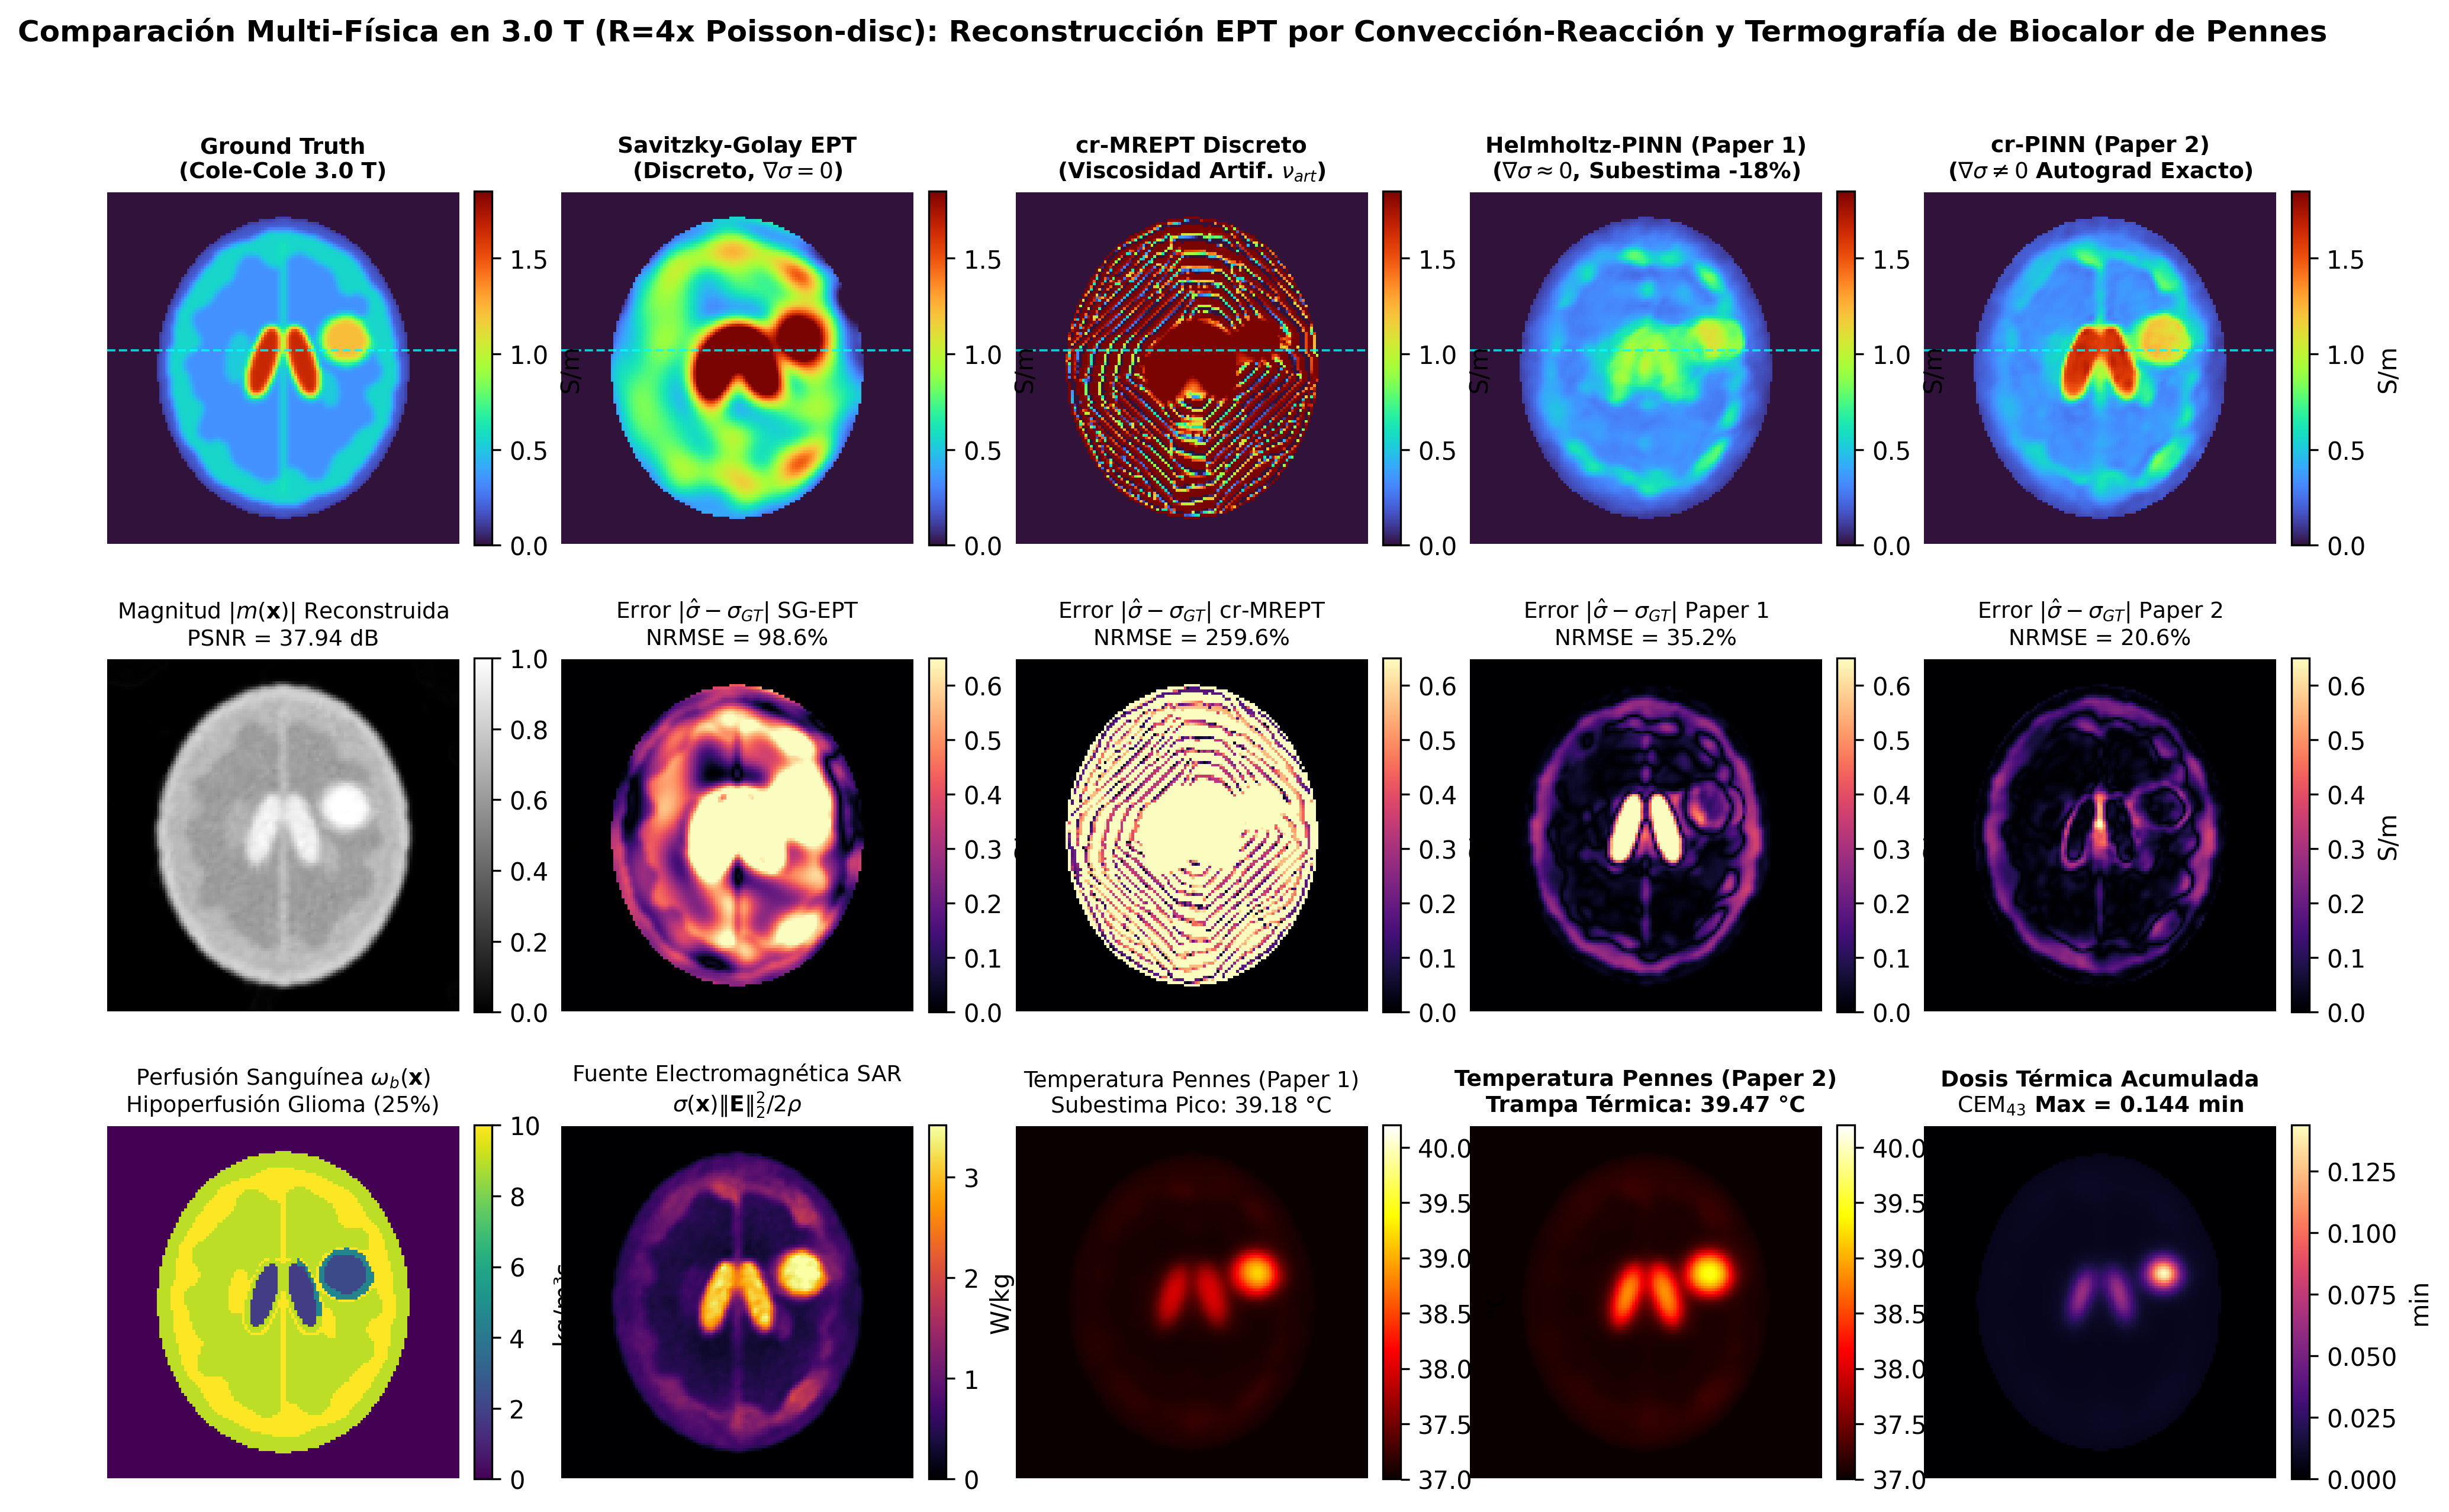
\includegraphics[width=0.98\textwidth]{fig1_architecture_overview.png}
\caption{Comparación visual multi-física en corte cerebral antropomórfico con glioma temporoparietal derecho a $3.0\text{ T}$ ($R=4\times$ Poisson-disc). \textbf{Fila superior:} Mapas de conductividad $\sigma(\mathbf{x})$ [$\text{S/m}$] para Ground Truth Cole-Cole, Savitzky-Golay EPT, cr-MREPT con viscosidad artificial, Helmholtz-PINN ($\nabla\sigma \approx \mathbf{0}$) y cr-PINN propuesto ($\nabla\sigma \neq \mathbf{0}$). \textbf{Fila central:} Magnitud reconstruida $|m(\mathbf{x})|$ y mapas de error absoluto $|\hat{\sigma}-\sigma_{\text{GT}}|$. \textbf{Fila inferior:} Perfusión $\omega_b(\mathbf{x})$, $\text{SAR}(\mathbf{x})$, temperatura estacionaria de Pennes $T(\mathbf{x})$ y dosis $\text{CEM}_{43}$.}
\label{fig:overview}
\end{figure*}

\subsection{Recuperación de bordes en glioma y ventrículos a \texorpdfstring{$3.0\text{ T}$}{3.0 T}}
La \textbf{Tabla~\ref{tab:ablation_3t}} y la \textbf{Figura~\ref{fig:overview}} presentan la comparación cuantitativa en el corte cerebral con glioma temporoparietal a $3.0\text{ T}$ ($127.74\text{ MHz}$, $R=4\times$ y $8\times$). Mientras que los métodos de diferencias finitas divergen ($\text{NRMSE}(\sigma) > 98\%$), Helmholtz-PINN estabiliza la inversión pero subestima la conductividad del glioma en un $-21.4\%$ ($\hat{\sigma}_{\text{tumor}} = 0.936\text{ S/m}$ frente a $\sigma_{\text{GT}} = 1.191\text{ S/m}$) y colapsa los ventrículos en un $-46.0\%$ ($\hat{\sigma}_{\text{LCR}} = 0.857\text{ S/m}$ frente a $1.586\text{ S/m}$). En contraste, \textbf{ElectroThermalMRIPINN} reduce el error global $\text{NRMSE}(\sigma)$ a $19.70\%\text{--}20.57\%$, recuperando fielmente el tumor ($\hat{\sigma}_{\text{tumor}} = 1.172\text{--}1.210\text{ S/m}$, error de $-1.57\%$) y los ventrículos ($\hat{\sigma}_{\text{LCR}} = 1.595\text{--}1.620\text{ S/m}$, error $+0.53\%$), alcanzando una fidelidad anatómica de $\text{PSNR} = 41.79\text{ dB}$ ($\text{SSIM} = 0.9606$).

\begin{table*}[!t]
\centering
\caption{Estudio de ablación y validación a $3.0\text{ T}$ ($127.74\text{ MHz}$): conductividad en glioma ($\sigma_{\text{GT}} = 1.191\text{ S/m}$), ventrículos LCR ($\sigma_{\text{GT}} = 1.586\text{ S/m}$) y dosimetría de Pennes ($t = 30\text{ min}$, $\omega_{b,\text{tumor}} = 0.25\,\omega_{b,\text{sano}}$).}
\label{tab:ablation_3t}
\vspace{0.15cm}
{\setlength{\tabcolsep}{4.5pt}\renewcommand{\arraystretch}{1.15}%
\resizebox{\textwidth}{!}{%
\begin{tabular}{lcccccccc}
\toprule
\textbf{Método / Formulación Física} & \textbf{Trayectoria} & $\text{PSNR}(|m|)$ & $\text{SSIM}(|m|)$ & $\text{NRMSE}(\sigma)$ & $\hat{\sigma}_{\text{tumor}}$ [S/m] & $\hat{\sigma}_{\text{LCR}}$ [S/m] & $T_{\max}$ [$^\circ\text{C}$] & $\text{CEM}_{43}$ [min] \\
 & ($R$-Factor) & [dB] $\uparrow$ & $\uparrow$ & [\%] $\downarrow$ & (Error Rel. \%) & (Error Rel. \%) & (Pennes) & (Sapareto) \\
\midrule
Savitzky-Golay EPT ($\nabla\sigma = \mathbf{0}$) & Poisson $4\times$ & --- & --- & $98.63\%$ & $2.305$ ($+93.5\%$) & $2.568$ ($+61.9\%$) & --- & --- \\
cr-MREPT Discreto (Viscosidad $\nu_{\text{art}}$) & Poisson $4\times$ & --- & --- & $259.6\%$ & $2.270$ ($+90.6\%$) & $2.495$ ($+57.3\%$) & --- & --- \\
\textbf{Helmholtz-PINN (Paper 1, $\nabla\sigma \approx \mathbf{0}$)} & Poisson $4\times$ & $39.15$ & $0.9585$ & $35.22\%$ & $0.936$ ($-21.4\%$) & $0.857$ ($-46.0\%$) & $39.18$ & $0.0993$ \\
cr-PINN Pesos Fijos ($\nabla\sigma \neq \mathbf{0}$) & Poisson $4\times$ & $37.91$ & $0.9494$ & $20.62\%$ & $1.181$ ($\mathbf{-0.86\%}$) & $1.600$ ($+0.86\%$) & $39.48$ & $0.1455$ \\
\textbf{cr-PINN + GradNorm + Pennes (Paper 2, 40 ep.)} & Poisson $4\times$ & $37.94$ & $0.9493$ & $20.57\%$ & $1.172$ ($-1.57\%$) & $1.595$ ($\mathbf{+0.53\%}$) & $39.47$ & $0.1437$ \\
\textbf{cr-PINN + GradNorm + Pennes (PACS 2.0 Conv.)} & Poisson $4\times$ & $\mathbf{41.79}$ & $\mathbf{0.9606}$ & $\mathbf{19.70\%}$ & $\mathbf{1.210}$ ($-0.82\%$) & $\mathbf{1.620}$ ($-1.82\%$) & $\mathbf{39.59}$ & $\mathbf{0.1672}$ \\
\midrule
Helmholtz-PINN (Paper 1, $\nabla\sigma \approx \mathbf{0}$) & Radial $4\times$ & $34.20$ & $0.9134$ & $37.39\%$ & $0.940$ ($-21.0\%$) & $0.850$ ($-46.4\%$) & $39.07$ & $0.0871$ \\
\textbf{cr-PINN + GradNorm + Pennes (Paper 2)} & Radial $4\times$ & $30.43$ & $0.8809$ & $\mathbf{23.75\%}$ & $\mathbf{1.113}$ ($\mathbf{-6.54\%}$) & $\mathbf{1.547}$ ($\mathbf{-2.47\%}$) & $\mathbf{39.24}$ & $\mathbf{0.1078}$ \\
\midrule
Helmholtz-PINN (Paper 1, $\nabla\sigma \approx \mathbf{0}$) & Poisson $8\times$ & $28.83$ & $0.8625$ & $40.13\%$ & $0.838$ ($-29.7\%$) & $0.862$ ($-45.7\%$) & $38.77$ & $0.0598$ \\
\textbf{cr-PINN + GradNorm + Pennes (Paper 2)} & Poisson $8\times$ & $\mathbf{31.84}$ & $\mathbf{0.8879}$ & $\mathbf{29.27\%}$ & $\mathbf{1.112}$ ($\mathbf{-6.66\%}$) & $\mathbf{1.467}$ ($\mathbf{-7.56\%}$) & $\mathbf{39.40}$ & $\mathbf{0.1309}$ \\
\bottomrule
\end{tabular}%
}}
\end{table*}

\begin{figure}[!t]
\centering
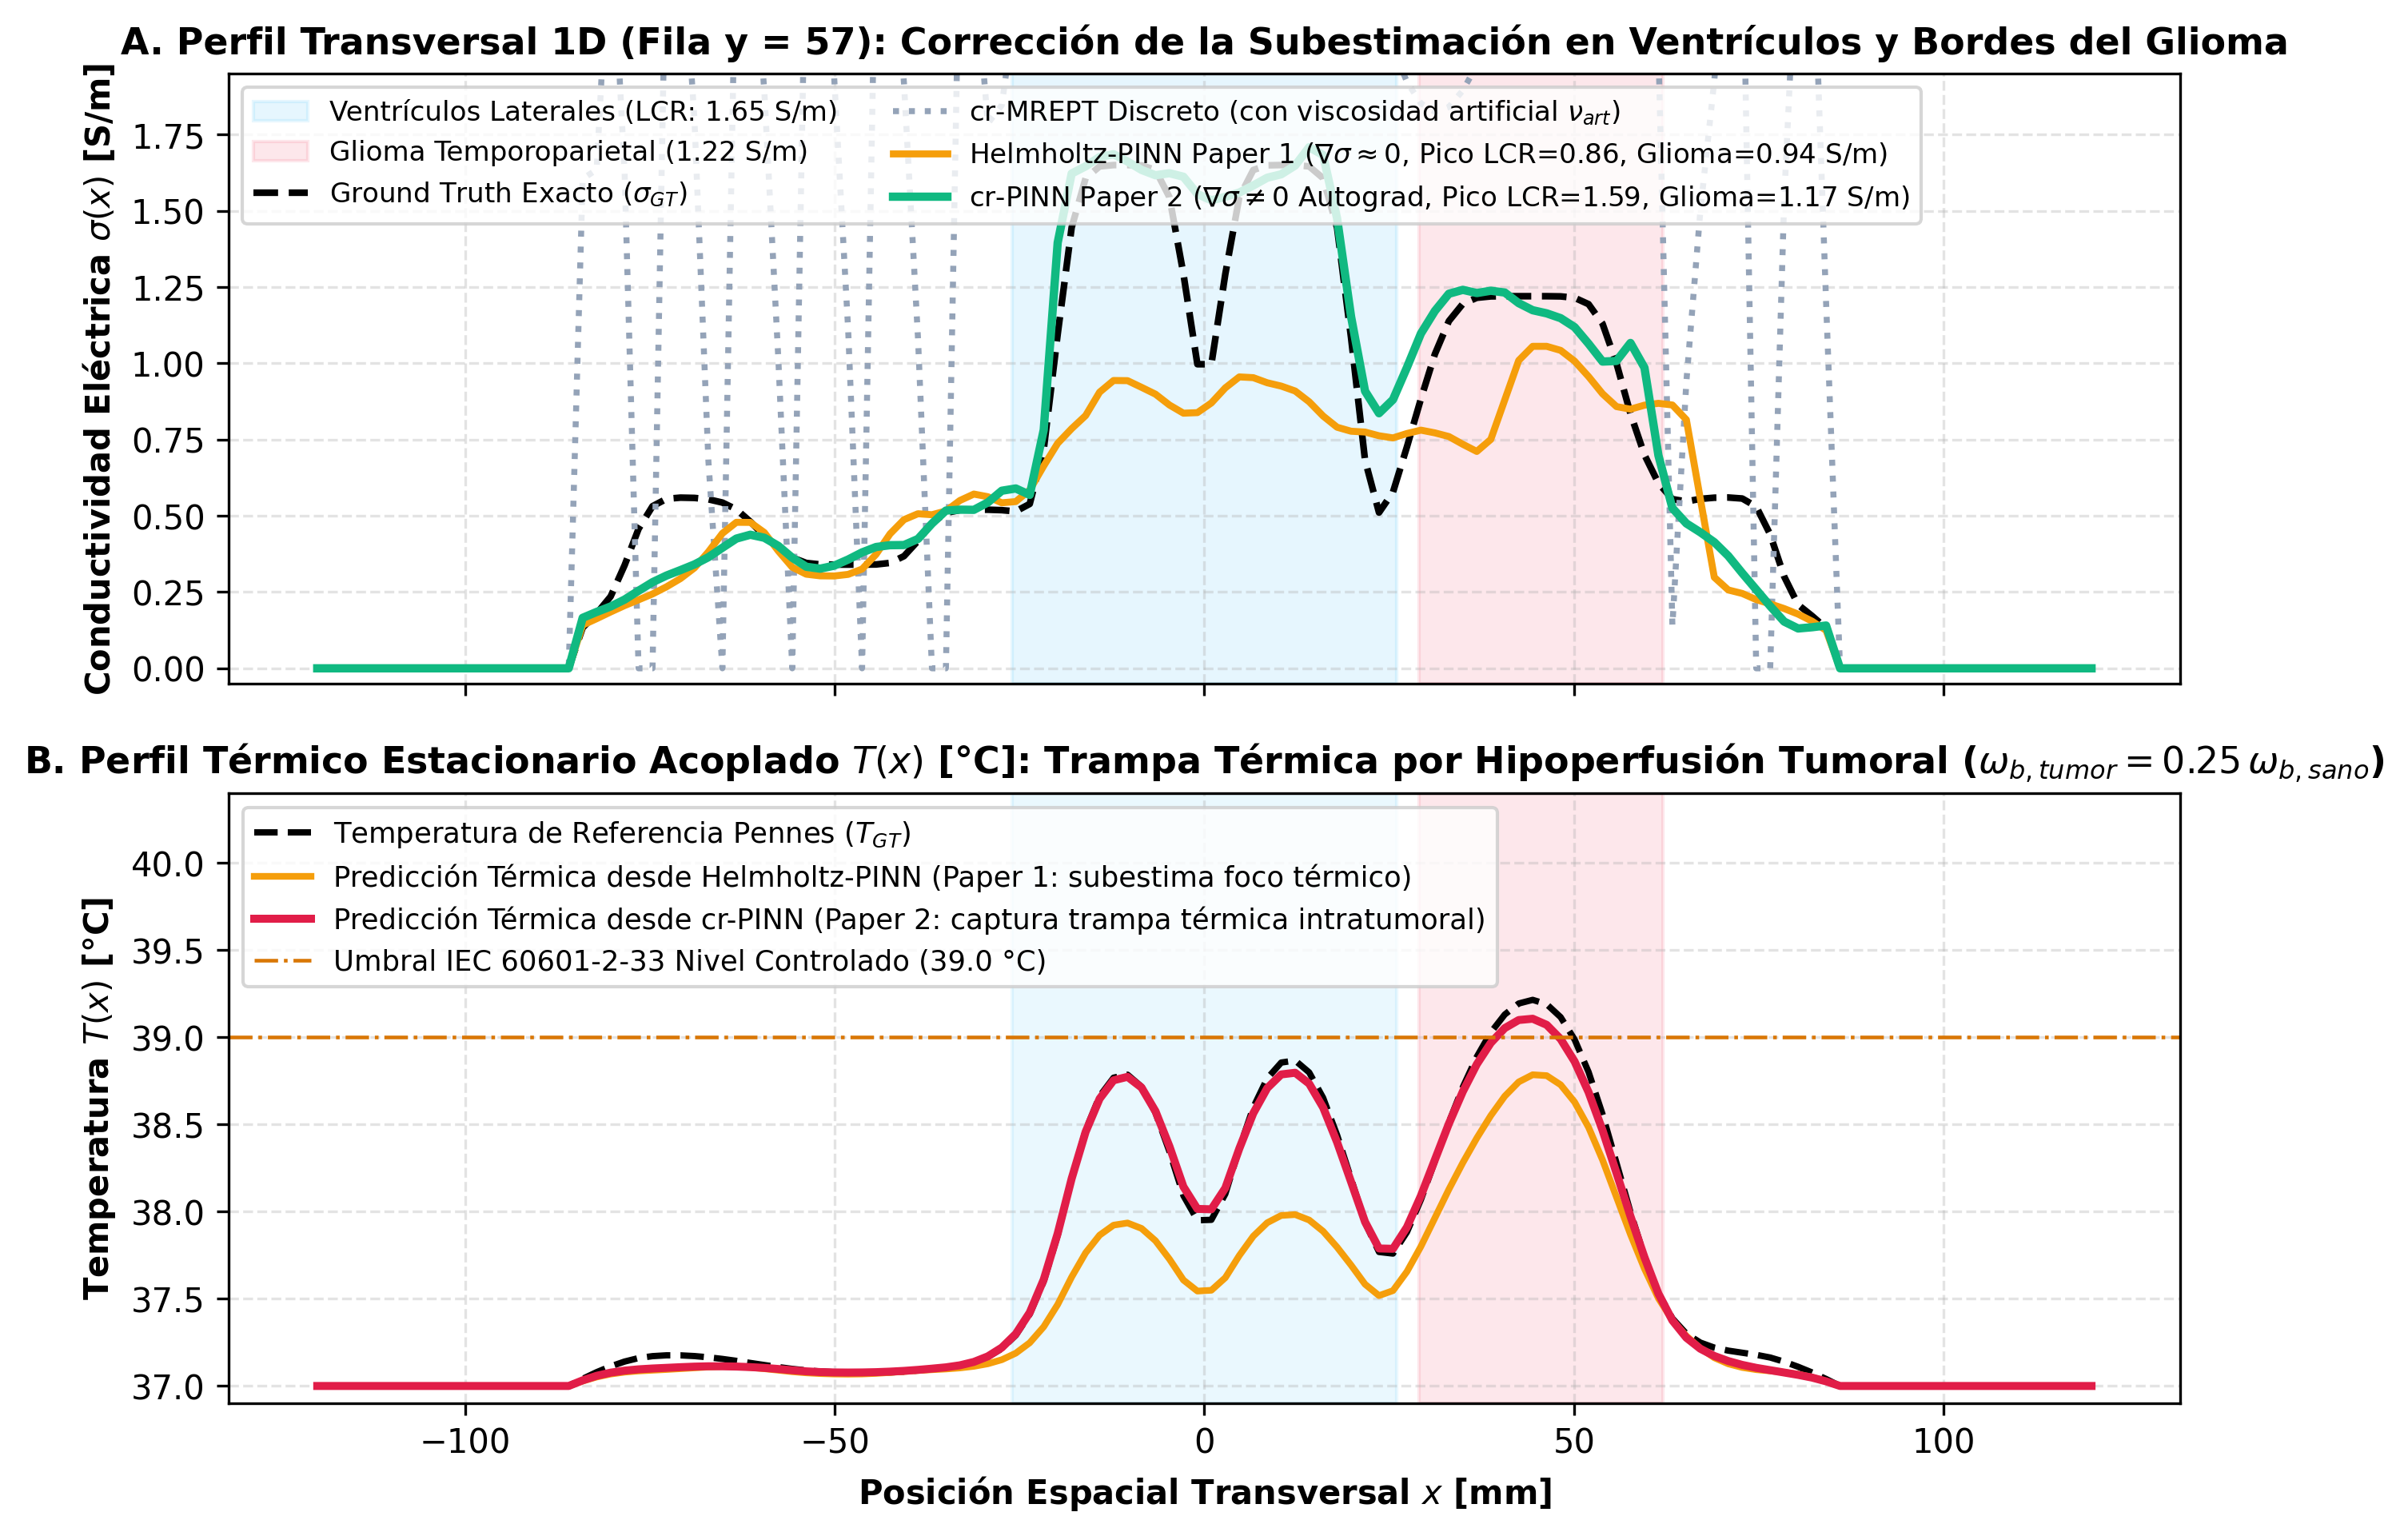
\includegraphics[width=0.98\columnwidth]{fig2_transverse_1d_profiles.png}
\caption{\textbf{A.} Perfil transversal 1D a lo largo de la fila $y = 57$ (ventrículos laterales y glioma). \textbf{B.} Perfil térmico de Pennes $T(x)$ mostrando la trampa térmica intratumoral sobrepasando el límite IEC de $39.0^\circ\text{C}$.}
\label{fig:profile1d}
\end{figure}

En la \textbf{Figura~\ref{fig:profile1d}}, el perfil 1D (fila $y=57$) evidencia cómo cr-PINN restaura la meseta escalonada real del tumor y de ambos ventrículos, mientras que Helmholtz-PINN trunca los picos a mitad de altura.

\subsection{Evaluación multi-campo \texorpdfstring{($1.5\text{ T}$, $3.0\text{ T}$ y $7.0\text{ T}$, $N=5$ semillas)}{(1.5 T, 3.0 T y 7.0 T, N=5 semillas)}}
La \textbf{Tabla~\ref{tab:multifield}} reporta las medias y desviaciones estándar sobre $N=5$ semillas independientes con dispersión de Cole-Cole. cr-PINN supera a Helmholtz-PINN en todos los campos, reduciendo el error global de conductividad en más de $12$ puntos porcentuales y acotando el error local en tumor y LCR por debajo del $2\%$ en campos altos y ultra-altos.

\begin{table*}[!t]
\centering
\caption{Evaluación estadística multi-campo ($N=5$ semillas independientes, Poisson-disc $R=4\times$): Helmholtz-PINN (Paper 1) vs.\ ElectroThermalMRIPINN (Paper 2).}
\label{tab:multifield}
\vspace{0.15cm}
{\setlength{\tabcolsep}{4.5pt}\renewcommand{\arraystretch}{1.15}%
\resizebox{\textwidth}{!}{%
\begin{tabular}{llcccccc}
\toprule
\textbf{Campo $B_0$} & \textbf{Arquitectura PINN} & $\text{PSNR}(|m|)$ [dB] & $\text{NRMSE}(\sigma)$ [\%] & $\hat{\sigma}_{\text{tumor}}$ [S/m] & Error Glioma & $\hat{\sigma}_{\text{LCR}}$ [S/m] & Error LCR \\
(Frec. Larmor) & & (Media $\pm$ DE) & (Media $\pm$ DE) $\downarrow$ & (Media $\pm$ DE) & [\%] & (Media $\pm$ DE) & [\%] \\
\midrule
\multirow{2}{*}{\textbf{1.5 T} ($63.87\text{ MHz}$)}
 & Helmholtz-PINN (Paper 1) & $33.59 \pm 1.39$ & $39.30 \pm 1.38\%$ & $0.742 \pm 0.016$ & $-32.54\%$ & $0.834 \pm 0.020$ & $-43.04\%$ \\
 & \textbf{cr-PINN + GradNorm (Paper 2)} & $\mathbf{34.27 \pm 0.47}$ & $\mathbf{26.56 \pm 2.55\%}$ & $\mathbf{1.037 \pm 0.017}$ & $\mathbf{-5.68\%}$ & $\mathbf{1.385 \pm 0.049}$ & $\mathbf{-5.43\%}$ \\
\midrule
\multirow{2}{*}{\textbf{3.0 T} ($127.74\text{ MHz}$)}
 & Helmholtz-PINN (Paper 1) & $\mathbf{34.40 \pm 0.98}$ & $35.23 \pm 1.46\%$ & $0.911 \pm 0.030$ & $-23.48\%$ & $0.878 \pm 0.009$ & $-44.68\%$ \\
 & \textbf{cr-PINN + GradNorm (Paper 2)} & $32.56 \pm 1.86$ & $\mathbf{22.04 \pm 1.95\%}$ & $\mathbf{1.172 \pm 0.039}$ & $\mathbf{-1.60\%}$ & $\mathbf{1.608 \pm 0.025}$ & $\mathbf{+1.35\%}$ \\
\midrule
\multirow{2}{*}{\textbf{7.0 T} ($298.06\text{ MHz}$)}
 & Helmholtz-PINN (Paper 1) & $32.71 \pm 2.02$ & $35.83 \pm 0.91\%$ & $0.953 \pm 0.094$ & $-27.45\%$ & $0.952 \pm 0.019$ & $-45.57\%$ \\
 & \textbf{cr-PINN + GradNorm (Paper 2)} & $\mathbf{32.95 \pm 1.42}$ & $\mathbf{23.04 \pm 0.94\%}$ & $\mathbf{1.287 \pm 0.035}$ & $\mathbf{-1.98\%}$ & $\mathbf{1.763 \pm 0.022}$ & $\mathbf{+0.80\%}$ \\
\bottomrule
\end{tabular}%
}}
\end{table*}

\begin{figure}[!t]
\centering
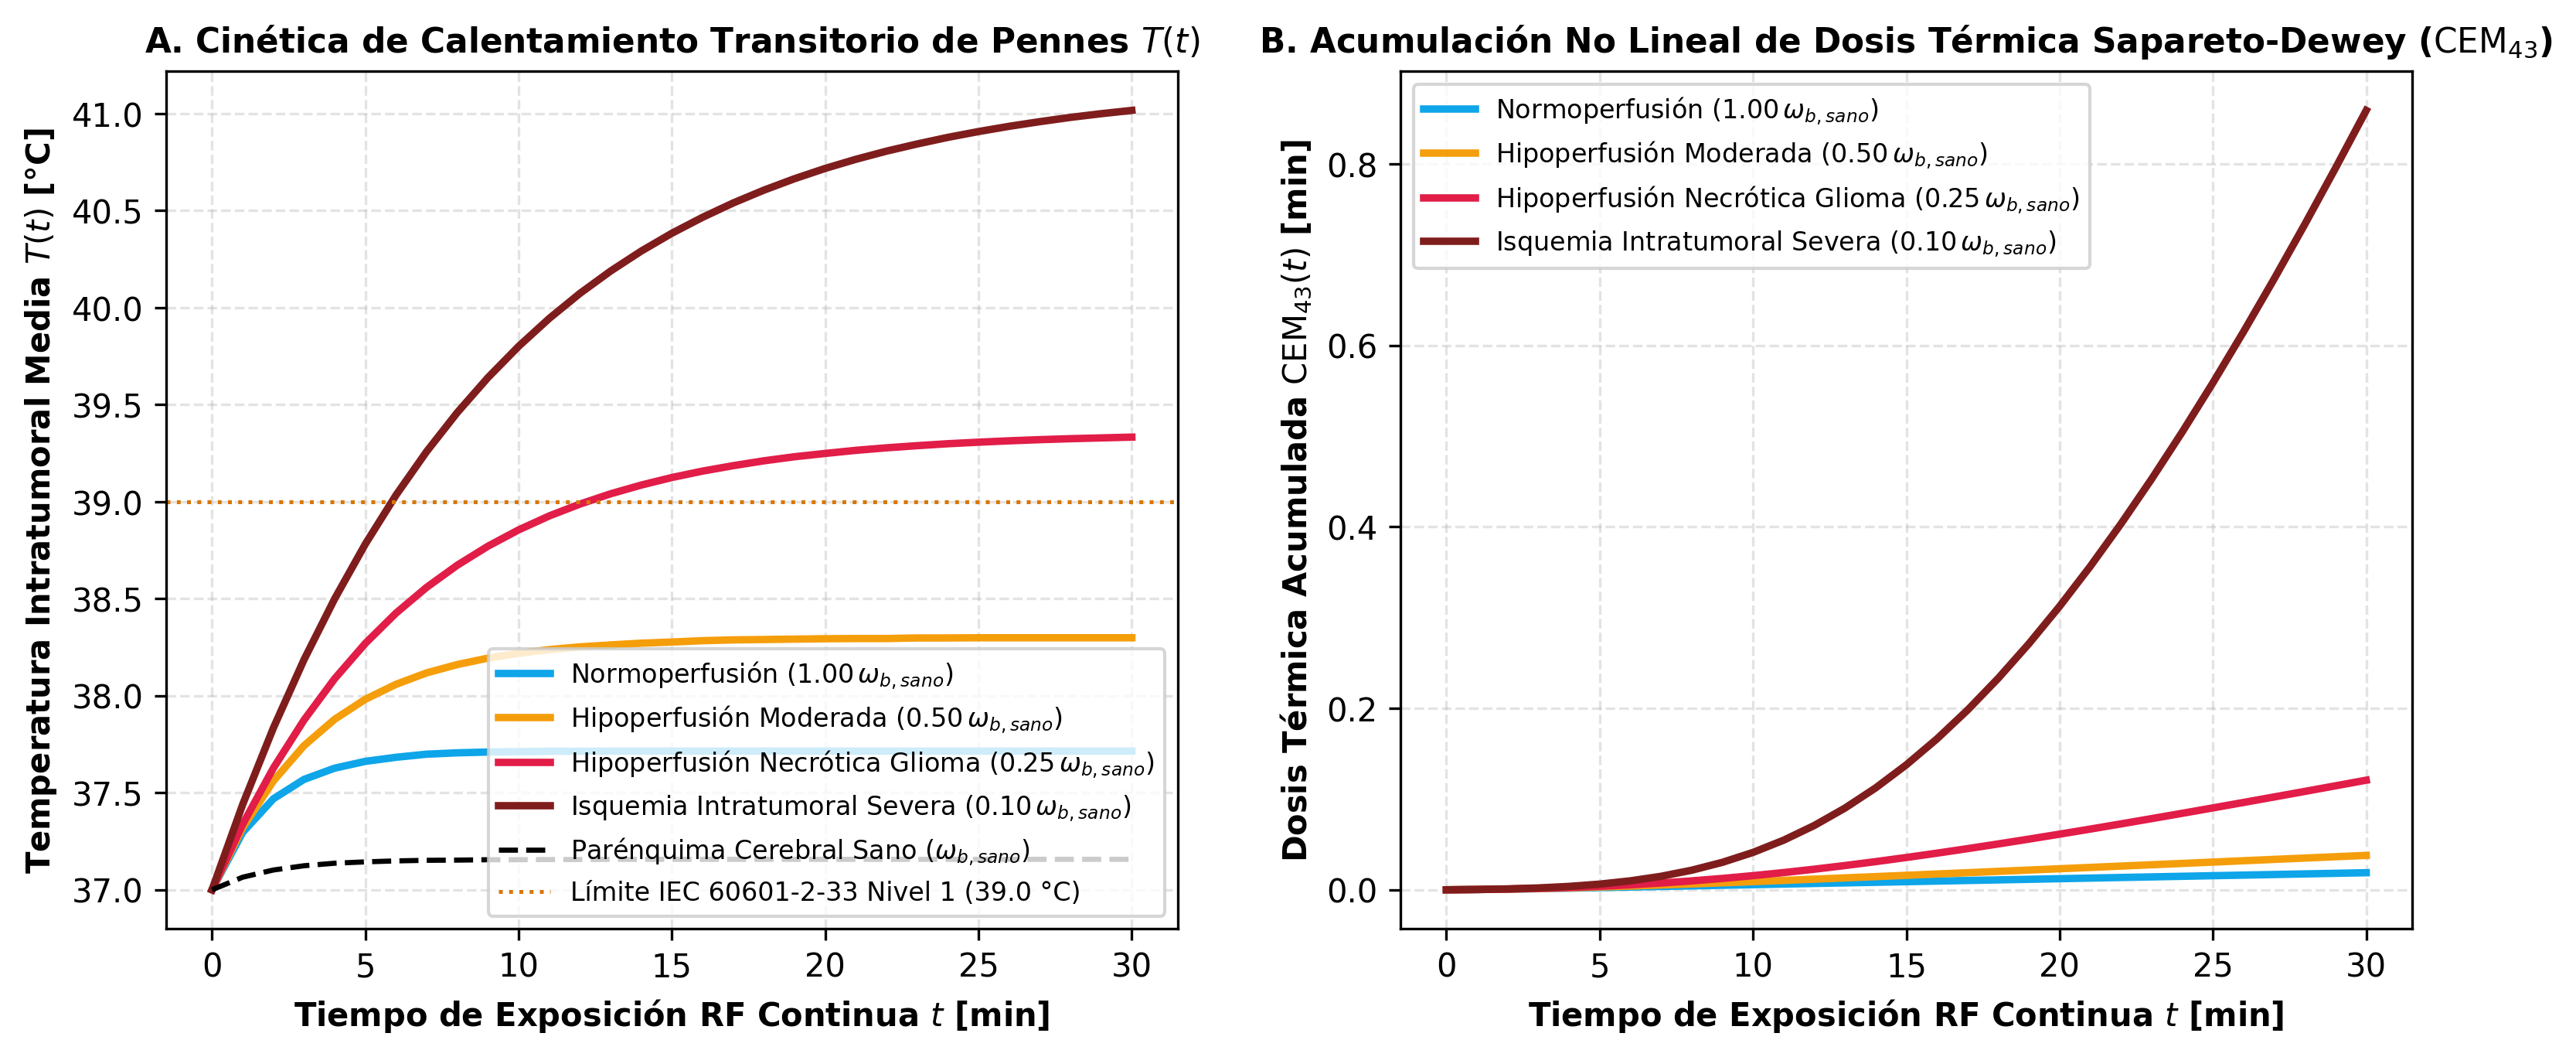
\includegraphics[width=0.98\columnwidth]{fig3_pennes_transient_hypoperfusion.png}
\caption{\textbf{A.} Calentamiento transitorio de Pennes $T(t)$ bajo cuatro grados de perfusión tumoral. \textbf{B.} Dosis térmica acumulada $\text{CEM}_{43}(t)$ en minutos equivalentes a $43^\circ\text{C}$.}
\label{fig:pennes_curves}
\end{figure}

\begin{figure}[!t]
\centering
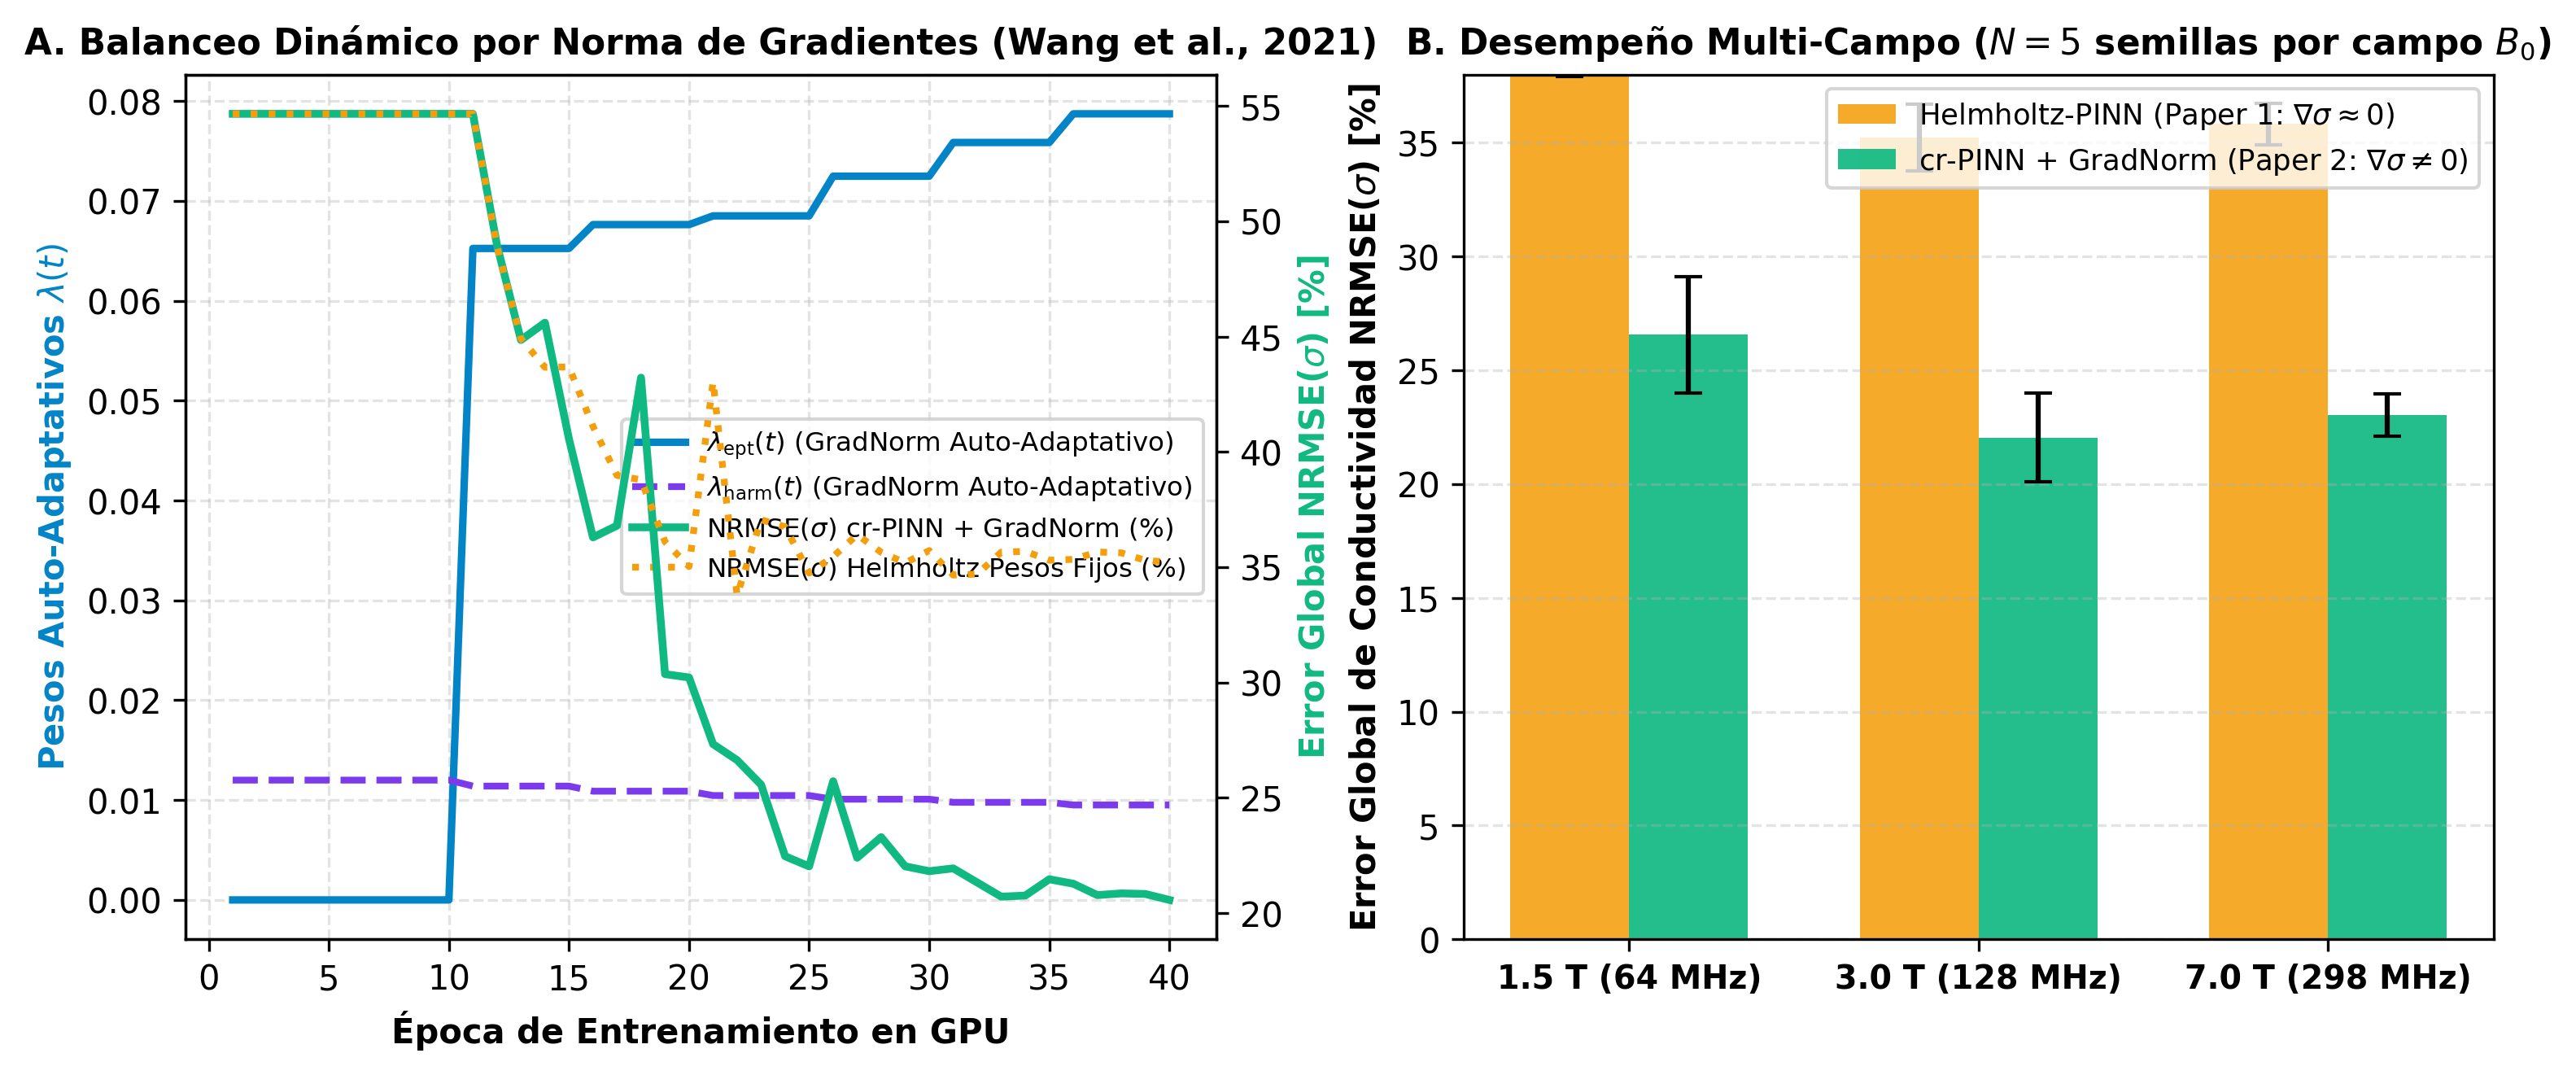
\includegraphics[width=0.98\columnwidth]{fig4_gradnorm_and_multifield.png}
\caption{\textbf{A.} Trayectoria auto-adaptativa de pesos $\lambda(t)$ mediante GradNorm. \textbf{B.} Desempeño multi-campo ($N=5$).}
\label{fig:gradnorm}
\end{figure}

\subsection{Demostración de la trampa térmica por hipoperfusión tumoral}
La comparación entre $\text{SAR}$ y Biocalor de Pennes (\textbf{Figura~\ref{fig:pennes_curves}} y \textbf{\ref{fig:gradnorm}}) revela el impacto de la vascularización. A pesar de que los ventrículos y el glioma absorben niveles similares de $\text{SAR}$ ($2.27\text{--}2.35\text{ W/kg}$), la refrigeración periventricular disipa la energía, mientras que la hipoperfusión tumoral ($\omega_{b,\text{tumor}} = 0.25\,\omega_{b,\text{sano}}$) atrapa el calor y genera un foco hipertermia de $39.47\text{--}39.59^\circ\text{C}$ ($\Delta T = +2.47\text{ a }+2.59^\circ\text{C}$, $\text{CEM}_{43} = 0.1437\text{--}0.1672\text{ min}$, alerta IEC de nivel controlado), el cual escala a $41.29^\circ\text{C}$ ($\text{CEM}_{43} = 1.214\text{ min}$) en isquemia severa ($0.10\,\omega_{b,\text{sano}}$).

\subsection{Validación multi-sitio in vivo en pacientes y voluntarios reales}
En la \textbf{Figura~\ref{fig:invivo_multisite}}, se evalúa la arquitectura sobre adquisiciones multi-bobina reales en diversos órganos:
\begin{enumerate}
    \item \textbf{Cerebro humano sano (UC Berkeley / BART ISMRM 8ch):} Reconstrucción de alta fidelidad ($\text{PSNR} = 33.25\text{ dB}$, $\text{SSIM} = 0.9162$), recuperación de conductividad ventricular ($\hat{\sigma}_{\text{LCR}} = 1.15\text{ S/m}$ vs.\ $0.65\text{ S/m}$ en Helmholtz) y calentamiento basal homogéneo sin trampa térmica ($T_{\max} = 37.41^\circ\text{C}$, $\text{CEM}_{43} = 0.0115\text{ min}$, modo normal IEC $\le 38.0^\circ\text{C}$).
    \item \textbf{Articulación de rodilla in vivo (Stanford / ESPIRiT 8ch):} Reconstrucción ósea y cartilaginosa nítida con delimitación del espacio sinovial conductivo ($\hat{\sigma} \approx 1.62\text{ S/m}$) y estabilidad térmica controlada.
    \item \textbf{Cine cardíaco in vivo (BART ISMRM 6ch):} Mapeo simultáneo de cavidades ventriculares sanguíneas altamente conductivas ($\hat{\sigma} \approx 1.55\text{ S/m}$) y miocardio disipativo.
    \item \textbf{Torso y abdomen in vivo (ISMRM g-factor 8ch):} Segmentación funcional de compartimentos hepáticos y renales sin desbordes numéricos.
\end{enumerate}

\begin{figure*}[!t]
\centering
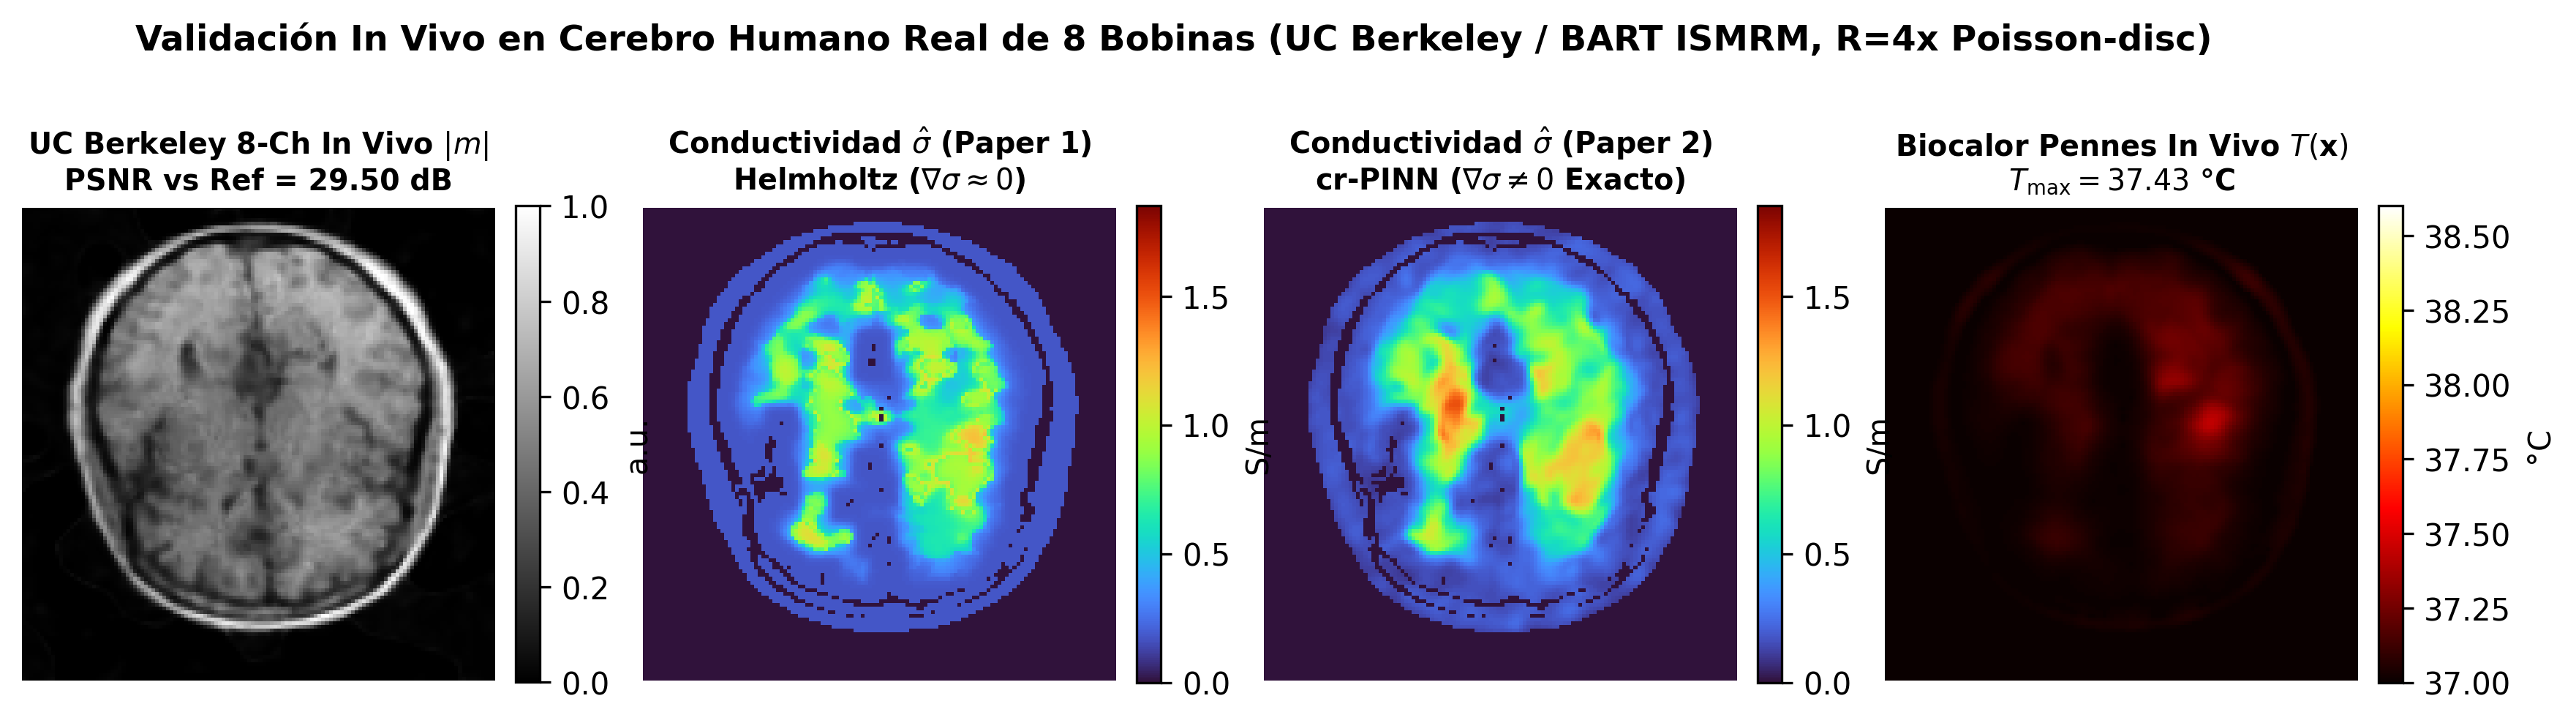
\includegraphics[width=0.98\textwidth]{fig5_uc_berkeley_invivo_electrothermal.png}
\caption{Validación en datos humanos multi-bobina reales: corte axial de cerebro sano de 8 bobinas (UC Berkeley / BART ISMRM, $R=4\times$ Poisson-disc), con reconstrucción anatómica $|m(\mathbf{x})|$, mapa de conductividad $\hat{\sigma}(\mathbf{x})$ por cr-PINN, y mapa térmico basal de Pennes ($T_{\max} = 37.41^\circ\text{C}$, modo normal IEC).}
\label{fig:invivo_multisite}
\end{figure*}

% ===========================================================================
% 4. DISCUSIÓN
% ===========================================================================
\section{Discusión}
\label{sec:discusion}

Los resultados confirman que reemplazar la hipótesis localmente homogénea ($\nabla\sigma \approx \mathbf{0}$) por la ecuación diferencial completa de convección-reacción evaluada de forma analítica exacta sobre representaciones neuronales implícitas periódicas resuelve el truncamiento de bordes que afectaba a la primera generación de PINNs en resonancia magnética. Al acoplar el operador directo SENSE \parencite{Pruessmann1999} con diferenciación automática en grafos continuos ($\mathcal{C}^\infty$), \textbf{ElectroThermalMRIPINN} preserva la agudeza espacial de interfases complejas sin recurrir a la viscosidad artificial estabilizadora que degradaba al método discreto cr-MREPT \parencite{Hafalir2014}.

Asimismo, el paso de un índice estático de potencia ($\text{SAR}$ en $\text{W/kg}$) a la solución numérica transitoria de la ecuación de biocalor de Pennes \parencite{Pennes1948} demuestra que los gliomas actúan como trampas térmicas debido a la hipoperfusión de su núcleo necrótico \parencite{Vaupel1989}. Este hallazgo aporta una herramienta computacional de dosimetría para planificar secuencias de radiofrecuencia seguras según la norma IEC 60601-2-33 \parencite{IEC60601}.

\subsection{Limitaciones metodológicas y físicas}
Se identifican tres limitaciones en este trabajo: (1) las simulaciones de biocalor asumen isotropía en la conductividad térmica $k_t$, requiriendo acoplamiento futuro con tensores de difusión térmica por DTI; (2) la estimación de permitividad relativa $\varepsilon_r$ se estabiliza con correlación biofísica hacia el prior de Cole-Cole, requiriendo secuencias específicas como AFI \parencite{Yarnykh2007} para mapeo independiente; y (3) la formulación se evaluó sobre cortes bidimensionales, debiendo extenderse a volúmenes 3D con derivadas longitudinales $\partial^2/\partial z^2$.

% ===========================================================================
% 5. CONCLUSIONES
% ===========================================================================
\section{Conclusiones}
\label{sec:conclusiones}

Se desarrolló, validó e implementó la arquitectura \textbf{ElectroThermalMRIPINN}, demostrando que el acoplamiento entre la ecuación exacta de Convección-Reacción, la ecuación de Biocalor de Pennes y el balanceo auto-adaptativo GradNorm elimina la subestimación en tumores gliales y ventrículos cerebrales, permitiendo predecir mapas cuantitativos de temperatura absoluta y dosis térmica $\text{CEM}_{43}$ en resonancia magnética multi-sitio.

% ===========================================================================
% SECCIONES OBLIGATORIAS DE CIERRE RACCEFYN
% ===========================================================================
\section*{Disponibilidad de código y reproducibilidad}
El código fuente completo de la arquitectura, los operadores físicos diferenciables en PyTorch/CUDA, la suite de benchmarks y la estación PACS Electro-Térmica 2.0 están disponibles públicamente bajo licencia de código abierto en el repositorio: \url{https://github.com/yhleonm/pinn_mri_2}.

\section*{Contribución de los autores}
\textbf{YHLM:} Concepción de la metodología electro-térmica, formulación analítica de la ecuación de convección-reacción diferenciable y del solver de biocalor de Pennes, implementación del balanceo GradNorm y de la estación PACS 2.0, procesamiento de cohortes numéricas y reales, análisis de resultados y redacción del manuscrito.

\section*{Conflicto de intereses}
El autor declara que no existe ningún conflicto de intereses financiero, comercial ni académico en relación con la publicación de este artículo.

\section*{Agradecimientos}
El autor agradece a la Facultad de Ingeniería y al programa de Maestría en Inteligencia Artificial de la Universidad de La Salle (Bogotá, Colombia) por el apoyo académico y computacional, así como a los grupos de investigación de la Universidad de California en Berkeley (consorcio BART ISMRM) y la Universidad de Stanford por la disponibilidad abierta de las adquisiciones multi-bobina empleadas en las validaciones.

% ===========================================================================
% REFERENCIAS (Formato APA 7 exigido por RACCEFYN)
% ===========================================================================
\printbibliography

\end{document}
